% Copyright (C) 2017 by SIB Swiss Institute of Bioinformatics, Julien Dorier and Dimos Goundaroulis.
% 
% This file is part of project Knoto-ID.
% 
% Knoto-ID is free software: you can redistribute it and/or modify
% it under the terms of the GNU General Public License as published by
% the Free Software Foundation, either version 2 of the License, or
% (at your option) any later version.
% 
% Knoto-ID is distributed in the hope that it will be useful,
% but WITHOUT ANY WARRANTY; without even the implied warranty of
% MERCHANTABILITY or FITNESS FOR A PARTICULAR PURPOSE.  See the
% GNU General Public License for more details.
% 
% You should have received a copy of the GNU General Public License
% along with Knoto-ID.  If not, see <http://www.gnu.org/licenses/>.

\section{\label{sec:reference}Command reference}

\subsection{Polynomial invariant}
\subsubsection{Usage}
\begin{lstlisting}
$ bin/polynomial_invariant [options] FILENAME
\end{lstlisting}

Load a piecewise linear curve from file  \lstinline{FILENAME}\footnote{in xyz file format, see section ``\ref{sec:format:xyz} \nameref{sec:format:xyz}'' for more information on the file format.}. To read from standard input instead, use file name \lstinline{stdin} or \lstinline{-}. By default, the curve is open (knotoid), but it can be closed (knot) by specifying a closure method with option \lstinline{--closure-method}. 
The input curve is then simplified using a 3D triangle elimination method\footnote{see section  ``\ref{sec:algorithms:3dsimplication} \nameref{sec:algorithms:3dsimplication}'' for more details.}.

Evaluate the knot(oid) diagram obtained by projecting the curve along  a randomly chosen projection direction (with uniform distribution on the surface of the sphere) or along the direction specified with option \lstinline{--projection}.
Alternatively, if \lstinline{--input-format=pd} or \lstinline{--input-format=gauss}, load directly the PD or extended Gauss code for a knot(oid) diagram from file \lstinline{FILENAME}.

Check that the knot(oid) diagram is valid using the method proposed by Vijayan and Wigderson\cite{Vijayan1982}.

Simplify the knot(oid) diagram with  Reidemeister moves\footnote{see section  ``\ref{sec:algorithms:diagramsimplication} \nameref{sec:algorithms:diagramsimplication}'' for more details.}.

Evaluate the polynomial invariant for the knot(oid) diagram on the surface of a sphere (by default) or on a plane (with option \lstinline{--planar}).

Output the polynomial invariant, and optionally the knot(oid) diagram\footnote{Output the simplified diagram.} (with option \lstinline{--output-diagram}).

If options \lstinline{--nb-projections} or  \lstinline{--projections-list} are used, the above procedure is repeated for all projections, and the output is a distribution of polynomials.

The polynomial invariant is the classical Jones polynomial for knots\cite{jones} when the curve in closed\\
(\lstinline{--closure-method=direct} or \lstinline{rays}), the Jones polynomial for knotoids\cite{turaev,guka} when the curve is open and the knotoid diagram is on the surface of a sphere (\lstinline{--closure-method=open}, without \lstinline{--planar}), and the Turaev loop bracket polynomial for knotoid\cite{turaev}  when the curve is open and the knotoid diagram is on the surface of a plane (\lstinline{--closure-method=open} and \lstinline{--planar}).


\subsubsection{Options}
\begin{description}
\item[\lstinline{-h}, \lstinline{--help}]\hfill\\
  Print usage.
\item[\lstinline{-V}, \lstinline{--version}]\hfill\\
  Print {\it Knoto-ID} version.
\item[\lstinline{-s SEED}, \lstinline{--seed=SEED}]\hfill\\
  Initialize the random number generator with  seed \lstinline{SEED}. If not specified, the seed is taken from the current time. 
\item[\lstinline{-F FORMAT}, \lstinline{--input-format=FORMAT}]\hfill\\
  Specify input format. Possible values for \lstinline{FORMAT}:
  \begin{itemize}
    \item \lstinline{xyz} piecewise linear curve in xyz file format\footnote{see section ``\ref{sec:format:xyz} \nameref{sec:format:xyz}'' for more information on the file format.}.
    \item \lstinline{pd} PD code for a knot(oid) diagram in KnotTheory file format\footnote{see section ``\ref{sec:format:pd} \nameref{sec:format:pd}''  for more information on the file format.}.  With input format \lstinline{pd}, options \lstinline{--projection}, \lstinline{--nb-projections}, \lstinline{--projections-list} and  \lstinline{--closure-method} are ignored. 
    \item \lstinline{gauss} extended Gauss code for a knot(oid) diagram\footnote{see section ``\ref{sec:format:gauss} \nameref{sec:format:gauss}''  for more information on the file format.}. Use option \lstinline{--closure-method=open} to specify that the diagram is open and \lstinline{--closure-method=direct} or \lstinline{rays} to specify that the diagram is  closed. With input format \lstinline{gauss}, options \lstinline{--projection}, \lstinline{--nb-projections} and \lstinline{--projections-list} are ignored. 
  \end{itemize}
  Default: \lstinline{xyz}.
\item[\lstinline{-o FILENAME}, \lstinline{--output=FILENAME}]\hfill\\
  Output the polynomial or distribution of polynomials to file \lstinline{FILENAME}.  To write to standard output, use file name \lstinline{stdout} or \lstinline{-}.\\
  Default \lstinline{stdout}.
\item[\lstinline{--output-diagram=FILENAME}]\hfill\\
  Output the knot(oid) diagram or list diagrams to  file \lstinline{FILENAME} using format specified with \lstinline{--output-diagram-format}. To write to standard output, use file name \lstinline{stdout} or \lstinline{-}.
\item[\lstinline{--output-diagram-format=FORMAT}]\hfill\\
  Specify output format for knot(oid) diagrams. Possible values for \lstinline{FORMAT}:
  \begin{itemize}
    \item \lstinline{pd} PD code for a knot(oid) diagram in KnotTheory file format\footnote{see section ``\ref{sec:format:pd} \nameref{sec:format:pd}''  for more information on the file format.}.  
    \item \lstinline{gauss} extended Gauss code for a knot(oid) diagram\footnote{see section ``\ref{sec:format:gauss} \nameref{sec:format:gauss}''  for more information on the file format.}.
  \end{itemize}
  Default: \lstinline{pd}.
\item[\lstinline{-m METHOD}, \lstinline{--closure-method=METHOD}]\hfill\\
  Specify how to close the input curve. Possible values for \lstinline{METHOD}:
  \begin{itemize}
  \item \lstinline{open} the curve is open (knotoid).
  \item \lstinline{direct} connect last point to first point by a straight line.
  \item \lstinline{rays} close by extending two parallel rays along the projection direction, each originating from one of the endpoints of the curve and connecting them outside the sphere that encloses the curve\footnote{see section ``\ref{sec:theory:knotoidsandcurves} \nameref{sec:theory:knotoidsandcurves}'' for more details.}.
  \end{itemize}
  Default: \lstinline{open}.
\item[\lstinline{-p}, \lstinline{--planar}]\hfill\\
  Evaluate polynomial invariant for the knot(oid) diagram on a plane. If not specified, evaluate polynomial invariant for the knot(oid) diagram on the surface of a sphere. This option is only relevant for open curves (\lstinline{--closure-method=open}).
\item[\lstinline{--nb-moves-III=NMOVES}]\hfill\\
  Use \lstinline{NMOVES} iterations to simplify the knot(oid) diagram using Reidemeister move III\footnote{see section  ``\ref{sec:algorithms:diagramsimplication} \nameref{sec:algorithms:diagramsimplication}'' for more details.}.\\
  Default \lstinline{100000}.
\item[\lstinline{--projection="X,Y,Z"}]\hfill\\ Project the input curve along projection direction (X,Y,Z). If not specified, use randomly chosen projection direction (with uniform distribution on the surface of the sphere).
\item[\lstinline{-N NPROJ}, \lstinline{--nb-projections=NPROJ}]\hfill\\
  Choose \lstinline{NPROJ} random projection directions (with uniform distribution on the surface of the sphere) and evaluate the corresponding polynomial invariant for each projection. Note:
  \begin{itemize}
  \item Instead of a unique polynomial, the output specified with \lstinline{--output} will contain the distribution of polynomials\footnote{see section ``\ref{sec:format:multiprojection:jones} \nameref{sec:format:multiprojection:jones}'' for more information on the file format.}. 
    \item The output specified with \lstinline{--output-diagram} will contain a list of projections with polynomials and knot(oid) diagrams\footnote{see section ``\ref{sec:format:multiprojection:diagrams} \nameref{sec:format:multiprojection:diagrams}'' for more information on the file format.}.
    \item For cyclic curves with closure method \lstinline{direct} the polynomial invariant (classical Jones polynomial) does not depend on the projection. To avoid useless computations \lstinline{NPROJ} will be set to 1.
    \item Option \lstinline{--projection} is ignored.                                  
  \end{itemize}
\item[\lstinline{--projections-list=FILENAME}]\hfill\\
  Load a list of projection directions from \lstinline{FILENAME}\footnote{see section ``\ref{sec:format:projections} \nameref{sec:format:projections}'' for more information on the file format.} and evaluate the corresponding polynomial invariant for each projection. Note:
  \begin{itemize}
  \item Instead of a unique polynomial, the output specified with \lstinline{--output} will contain the distribution of polynomials\footnote{see section ``\ref{sec:format:multiprojection:jones} \nameref{sec:format:multiprojection:jones}'' for more information on the file format.}. 
    \item The output specified with \lstinline{--output-diagram} will contain a list of projections with polynomials and knot(oid) diagrams\footnote{see section ``\ref{sec:format:multiprojection:diagrams} \nameref{sec:format:multiprojection:diagrams}'' for more information on the file format.}.
    \item For cyclic curves with closure method \lstinline{direct} the polynomial invariant (classical Jones polynomial) does not depend on the projection. To avoid useless computations, only one projection direction will be used.
    \item Options  \lstinline{--nb-projections} and \lstinline{--projection} are ignored.                                  
  \end{itemize}
\item[\lstinline{-n FILENAME}, \lstinline{--names-db=FILENAME}]\hfill\\
  Load a list of polynomials with corresponding knot(oid) names from file \lstinline{FILENAME}\footnote{see section ``\ref{sec:format:namesdb} \nameref{sec:format:namesdb}'' for more information on the file format.}.
\item[\lstinline{--timeout=TIMEOUT}]\hfill\\
  Abort evaluation of polynomial invariant after \lstinline{TIMEOUT} seconds (integer number). Note: if the evaluation of the polynomial invariant is aborted, the polynomial is replaced by \lstinline{TIMEOUT}.
\end{description}


      
\subsection{Knotted core}
\subsubsection{Usage}
\begin{lstlisting}
$ bin/knotted_core [options] FILENAME
\end{lstlisting}

Load a piecewise linear curve from file  \lstinline{FILENAME}\footnote{in xyz file format, see section ``\ref{sec:format:xyz} \nameref{sec:format:xyz}''  for more information on the file format.} and evaluate the knotted core\footnote{see section  ``\ref{sec:algorithms:knottedcore} \nameref{sec:algorithms:knottedcore}'' for more information on the file format.}.
To read from standard input instead, use file name \lstinline{stdin} or \lstinline{-}.
By default, the curve is considered open, but it can be closed with option \lstinline{--cyclic-input}.

Output the knotted core,  and optionally all subchains tested when searching the knotted core (with option \lstinline{--output-search}) as well as all possible subchains of the input curve (with option \lstinline{--output-all}).

Note that the knotted core corresponds to the "top-down" knotted core discussed by Tubiana and coauthors \cite{tubiana2011}.

\subsubsection{Options}
\begin{description}
\item[\lstinline{-h}, \lstinline{--help}]\hfill\\
  Print usage.
\item[\lstinline{-V}, \lstinline{--version}]\hfill\\
  Print {\it Knoto-ID} version.
\item[\lstinline{-s SEED}, \lstinline{--seed=SEED}]\hfill\\
  Initialize the random number generator with  seed \lstinline{SEED}. If not specified, the seed is taken from the current time. 
\item[\lstinline{-o FILENAME}, \lstinline{--output=FILENAME}]\hfill\\
  Output the knotted core to file \lstinline{FILENAME}\footnote{see section ``\ref{sec:format:listsubchains} \nameref{sec:format:listsubchains}'' for more information on the file format.}.  To write to standard output, use file name \lstinline{stdout} or \lstinline{-}.\\
  Default \lstinline{stdout}.
\item[\lstinline{--output-search=FILENAME}]\hfill\\
  Output all subchains tested when searching for the knotted core to file \lstinline{FILENAME}\footnote{see section ``\ref{sec:format:listsubchains} \nameref{sec:format:listsubchains}'' for more information on the file format.}. To write to standard output, use file name \lstinline{stdout} or \lstinline{-}.
\item[\lstinline{--output-all=FILENAME}]\hfill\\
  Output all possible subchains of the input curve to file \lstinline{FILENAME}\footnote{see section ``\ref{sec:format:listsubchains} \nameref{sec:format:listsubchains}'' for more information on the file format.}. To write to standard output, use file name \lstinline{stdout} or \lstinline{-}. Warning: evaluating the polynomial invariants for all subchains of the input curve may be slow.
\item[\lstinline{-C}, \lstinline{--cyclic-input}]\hfill\\
  Close the input curve by connecting its last point to its first point by a straight line.  
\item[\lstinline{-m METHOD}, \lstinline{--closure-method=METHOD}]\hfill\\
  Specify how to close each subchain. Possible values for \lstinline{METHOD}:
  \begin{itemize}
  \item \lstinline{open} the subchain is open (knotoid).
  \item \lstinline{direct} connect last point to first point by a straight line.
  \item \lstinline{rays} close by extending two parallel rays along the projection direction, each originating from one of the endpoints of the curve and connecting them outside the sphere that encloses the curve\footnote{see section ``\ref{sec:theory:knotoidsandcurves} \nameref{sec:theory:knotoidsandcurves}'' for more details.}.
  \end{itemize}
  Default: \lstinline{open}.
\item[\lstinline{-p}, \lstinline{--planar}]\hfill\\
  For each subchain, evaluate its polynomial invariant for the knot(oid) diagram on a plane. If not specified, evaluate polynomial invariant for the knot(oid) diagram on the surface of a sphere. This option is only relevant for open curves (\lstinline{--closure-method=open}).
\item[\lstinline{--nb-moves-III=NMOVES}]\hfill\\
  Use \lstinline{NMOVES} iterations to simplify the knot(oid) diagram using Reidemeister move III\footnote{see section  ``\ref{sec:algorithms:diagramsimplication} \nameref{sec:algorithms:diagramsimplication}'' for more details.}.\\
  Default \lstinline{10}.
\item[\lstinline{-N NPROJ}, \lstinline{--nb-projections=NPROJ}]\hfill\\
  Use \lstinline{NPROJ} random projection directions (with uniform distribution on the surface of the sphere) to evaluate the dominant polynomial invariant of each subchain.  For cyclic subchains with closure method \lstinline{direct} the polynomial invariant (classical Jones polynomial) does not depend on the projection. To avoid useless computations \lstinline{NPROJ} will be set to 1.\\
  Default: \lstinline{20}.
\item[\lstinline{--projections-list=FILENAME}]\hfill\\
 Evaluate the dominant polynomial using the list of projection directions in file \lstinline{FILENAME}\footnote{see section ``\ref{sec:format:projections} \nameref{sec:format:projections}''  for more information on the file format.}. Note:
  \begin{itemize}
    \item For cyclic subchains with closure method \lstinline{direct} the polynomial invariant (classical Jones polynomial) does not depend on the projection. To avoid useless computations, only one projection direction will be used.
    \item Options  \lstinline{--nb-projections} is ignored.                                  
  \end{itemize}
\item[\lstinline{-n FILENAME}, \lstinline{--names-db=FILENAME}]\hfill\\
  Load a list of polynomials with corresponding knot(oid) names from file \lstinline{FILENAME}\footnote{see section ``\ref{sec:format:namesdb} \nameref{sec:format:namesdb}'' for more information on the file format.}.
\item[\lstinline{--timeout=TIMEOUT}]\hfill\\
  Abort evaluation of polynomial invariant after \lstinline{TIMEOUT} seconds (integer number). Note: if the evaluation of the polynomial invariant is aborted, the polynomial is replaced by \lstinline{TIMEOUT}.
\end{description}

\subsection{Convert diagram}
\subsubsection{Usage}
\begin{lstlisting}
$ bin/convert_diagram [options] FILENAME
\end{lstlisting}


Load a knot(oid) diagram file \lstinline{FILENAME}. To read from standard input instead, use file name \lstinline{stdin} or \lstinline{-}.

Depending on \lstinline{--input-format}, different types of files can be opened:
\begin{itemize}
\item If  \lstinline{--input-format=pd} (by default), load the diagram in PD code format \footnote{see section ``\ref{sec:format:pd} \nameref{sec:format:pd}''  for more information on the file format.}.
\item If  \lstinline{--input-format=gauss}, load the diagram in extended Gauss code format\footnote{see section ``\ref{sec:format:gauss} \nameref{sec:format:gauss}''  for more information on the file format.}. Option \lstinline{--closure-method} is used to specify whether the diagram is open (default) or closed.
\item If  \lstinline{--input-format=xyz}, load a piecewise linear curve in xyz format\footnote{see section ``\ref{sec:format:xyz} \nameref{sec:format:xyz}'' for more information on the file format.}. 
  By default, the curve is open (knotoid), but it can be closed (knot) by specifying a closure method with option \lstinline{--closure-method}.
  If option \lstinline{--3D-reduction} is given, the input curve is simplified using a 3D triangle elimination method\footnote{see section  ``\ref{sec:algorithms:3dsimplication} \nameref{sec:algorithms:3dsimplication}'' for more details.}.
  
  A knot(oid) diagram is then obtained by projecting the curve along a randomly chosen projection direction (with uniform distribution on
  the surface of the sphere) or along the direction specified with  option \lstinline{--projection}.  
\end{itemize}
Check that the knot(oid) diagram is valid using the method proposed by Vijayan and Wigderson\cite{Vijayan1982}.


If option \lstinline{--simplify-diagram} is given, the knot(oid) diagram is simplified using Reidemeister moves.
Finally, the resulting diagram is saved to file specified by option \lstinline{--output}, with format specified by \lstinline{--output-format}.

Notes:
\begin{itemize}
\item If the input is in xyz format or contains information on which arcs
  touch the outside region, option \lstinline{--planar} can be used to keep this information 
  in the output.
\item To output in ``xyz for knot(oid) diagram`` format, \lstinline{convert_diagram} uses a circle packing algorithm\footnote{see section ``\ref{sec:algorithms:circlepacking} \nameref{sec:algorithms:circlepacking}'' for more information.} to draw the diagram in the x-y plane (with z storing information on what stand is above/below in each crossing). While this algorithm usually produces good results for knot diagrams (see Figures \ref{fig:diagram1} and \ref{fig:diagram2}), it may also produce poorly balanced results, with circle radii (or arc lengths) differing by several orders of magnitude. This problem of unbalanced circle packing is particularly strong for planar knotoid diagrams, in particular when the diagram is enclosed within an external loop. To mitigate this problem, it is possible to use a simulated annealing algorithm to ``relax'' the diagram (with option \lstinline{--nb-iterations-relaxation}).
  By default, if the resulting diagram is not balanced (i.e. ratio of largest arc length to shortest arc length is larger than 20), \lstinline{convert_diagram} will quit with an error without writing the resulting diagram (to avoid producing unreadable and potentially misleading output). To ignore this test and write the diagram even if it is unbalanced, use option \lstinline{--force}.
\end{itemize}


\subsubsection{Options}
\begin{description}
\item[\lstinline{-h}, \lstinline{--help}]\hfill\\
  Print usage.
\item[\lstinline{-V}, \lstinline{--version}]\hfill\\
  Print {\it Knoto-ID} version.
\item[\lstinline{-s SEED}, \lstinline{--seed=SEED}]\hfill\\
  Initialize the random number generator with  seed \lstinline{SEED}. If not specified, the seed is taken from the current time. 
\item[\lstinline{-p}, \lstinline{--planar}]\hfill\\
  Use information on what arcs are touching the outside region.
  
  WARNING: exit with error if the input file does not contain this information.
\item[\lstinline{-F FORMAT}, \lstinline{--input-format=FORMAT}]\hfill\\
  Specify input format. Possible values for \lstinline{FORMAT}:
  \begin{itemize}
  \item \lstinline{xyz} piecewise linear curve in xyz file format\footnote{see section ``\ref{sec:format:xyz} \nameref{sec:format:xyz}'' for more information on the file format.}.
  \item \lstinline{pd} PD code for a knot(oid) diagram in KnotTheory file format\footnote{see section ``\ref{sec:format:pd} \nameref{sec:format:pd}''  for more information on the file format.}.  With input format \lstinline{pd}, options \lstinline{--projection} and  \lstinline{--closure-method} are ignored. 
    If the input file contains multiple PD codes, only the first one will be used.
  \item \lstinline{gauss} extended Gauss code for a knot(oid) diagram\footnote{see section ``\ref{sec:format:gauss} \nameref{sec:format:gauss}''  for more information on the file format.}. Use option \lstinline{--closure-method=open} to specify that the diagram is open and \lstinline{--closure-method=direct} or \lstinline{rays} to specify that the diagram is closed. With input format \lstinline{gauss}, option \lstinline{--projection} is ignored.
    If the input file contains multiple Gauss codes, only the first one will be used.
  \end{itemize}
  Default: \lstinline{xyz}.
\item[\lstinline{--output-format=FORMAT}]\hfill\\
  Specify output format. Possible values for \lstinline{FORMAT}:
  \begin{itemize}
  \item \lstinline{pd} PD code for knot(oid) diagrams\footnote{see section ``\ref{sec:format:pd} \nameref{sec:format:pd}''  for more information on the file format.}. 
  \item \lstinline{gauss} extended Gauss code for knot(oid) diagrams\footnote{see section ``\ref{sec:format:gauss} \nameref{sec:format:gauss}''  for more information on the file format.}.
  \item \lstinline{xyz} xyz format for knot(oid) diagrams\footnote{see section ``\ref{sec:format:xyzdiagrams} \nameref{sec:format:xyzdiagrams}'' for more information on the file format.}.
  \end{itemize}
  Default: \lstinline{pd}.
\item[\lstinline{-o FILENAME}, \lstinline{--output=FILENAME}]\hfill\\
  Output the knot(oid) diagram to file \lstinline{FILENAME} using format specified with \lstinline{--output-format}.  To write to standard output, use file name \lstinline{stdout} or \lstinline{-}.\\
  Default \lstinline{stdout}.
  %options for diagram simplification
\item[\lstinline{--simplify-diagram}]\hfill\\
  Simplify the knot(oid) diagram using Reidemeister moves.
\item[\lstinline{--nb-moves-III=NMOVES}]\hfill\\
  Use \lstinline{NMOVES} iterations to simplify the knot(oid) diagram using Reidemeister move III\footnote{see section  ``\ref{sec:algorithms:diagramsimplication} \nameref{sec:algorithms:diagramsimplication}'' for more details.}.\\
  Default \lstinline{100000}.
  %options for xyz input format
\end{description}
\paragraph{Options for xyz input format:}
\begin{description}
\item[\lstinline{-m METHOD}, \lstinline{--closure-method=METHOD}]\hfill\\
  Specify how to close the input curve. Possible values for \lstinline{METHOD}:
  \begin{itemize}
  \item \lstinline{open} the curve is open (knotoid).
  \item \lstinline{direct} connect last point to first point by a straight line.
  \item \lstinline{rays} close by extending two parallel rays along the projection direction, each originating from one of the endpoints of the curve and connecting them outside the sphere that encloses the curve\footnote{see section ``\ref{sec:theory:knotoidsandcurves} \nameref{sec:theory:knotoidsandcurves}'' for more details.}.
  \end{itemize}
  Only used with \lstinline{--input-format=xyz} and \lstinline{gauss}.\\
  Default: \lstinline{open}.  
\item[\lstinline{--projection="X,Y,Z"}]\hfill\\
  Project the input curve along projection direction (X,Y,Z). If not specified, use randomly chosen projection direction (with uniform distribution on the surface of the sphere). Only used with \lstinline{--input-format=xyz}.
\item[\lstinline{--3D-reduction}]\hfill\\
  Simplify the input curve using a 3D triangle elimination method\footnote{see section  ``\ref{sec:algorithms:3dsimplication} \nameref{sec:algorithms:3dsimplication}'' for more details.}. Only used with \lstinline{--input-format=xyz}.
\end{description}
\paragraph{Options for xyz output format:}
\begin{description}
\item[\lstinline{--force}]\hfill\\
  Output the knot(oid) diagram without checking if it is balanced (i.e. same order of magnitude for all arc lengths).
  Without \lstinline{--force}, quit without saving the diagram if it is not balanced.
\item[\lstinline{--nb-iterations-relaxation=N}]\hfill\\
  After circle packing, relax the knot(oid) diagram with N iterations of simulated annealing.\\
  Default: \lstinline{0}.  
\end{description}


\subsection{\label{sec:algorithms}Algorithms}
In the following the main algorithms used in {\it Knoto-ID} are briefly described.

\subsubsection{\label{sec:algorithms:3dsimplication}Curve simplification using triangle elimination}
Evaluating a polynomial invariant can be very challenging  since the run time scales exponentially with the number of crossings in the knot(oid) diagram. Therefore, one needs to reduce as much as possible the number of crossings. One way to achieve this goal consists in simplifying the 3D curve used as input, without modifying its topology, before evaluating its knot(oid) diagram. To do this, we use a triangle elimination method based on the KMT algorithm\cite{Koniaris1991}\cite{taylor2000}: For each triplet of sequential points along the curve, if the triangle formed by the three points is not crossed by any segment of the curve, the middle point is removed and the first and last point of the triplet are directly connected by a straight line.
This operation is repeated iteratively until no point of the curve can be removed.
When the input curve is open (knotoid), we first introduce two infinite lines that pass through the endpoints of the curve, parallel to the direction of projection. The same algorithm is then used with a small modification: a point is removed only if the triangle is not crossed by any segment of the curve nor by any infinite line.

\subsubsection{\label{sec:algorithms:diagramsimplication}Knot(oid) diagram simplification}
The next step of simplification is performed directly on the knot(oid) diagram.

\paragraph{Simplification with type I and II Reidemeister moves.}
The knot(oid) diagram is simplified by iteratively applying type I and II Reidemeister moves\footnote{see Figure~\ref{fig:rmoves} in section ``\ref{sec:format:namesdb} \nameref{sec:format:namesdb}''.} that decrease the number of crossings until no more crossings can be removed.

\paragraph{Random shuffling with type III Reidemeister.}
Among all possible type III Reidemeister moves that can be applied to the knot(oid) diagram, one move is randomly chosen and applied to the diagram.
This operation is followed by a simplification with  type I and II Reidemeister moves described previously.
The combination of Random shuffling with type III Reidemeister followed by a simplification with  type I and II Reidemeister moves is then repeated multiple times (specified with \lstinline{--nb-moves-III}).

While the simplification method can strongly reduce the complexity of the knot(oid) diagram, and therefore the computational time, it introduces an overhead that can become non-negligible for relatively simple diagrams. Therefore it may be worth adjusting the number of iterations with \lstinline{--nb-moves-III} to find the optimal balance between computational effort spent in the simplification of the knot(oid) diagram and in the evaluation of the polynomial invariant.


\subsubsection{\label{sec:algorithms:jonespolynomial}Polynomial invariant}
The polynomial invariants are evaluated by recursively applying the skein relations discussed in section ``\ref{sec:theory:jones} \nameref{sec:theory:jones}'' to all crossings of the knot(oid) diagram. At each step of the recursion, the resulting diagram is simplified by type I and II Reidemeister moves whenever possible, thus reducing the number of iteration in the recursion. Although the run time of this algorithm still scales exponentially with the number of crossings in the diagram, the simplification by type I and II Reidemeister moves reduces the execution time by a factor that increase exponentially with the number of crossings.


\subsubsection{\label{sec:algorithms:knottedcore}Knotted core}
The knotted core is defined as the shortest subchain obtained by progressively altering the length of the whole curve by 1 point without changing the knot(oid) type in the process.
When the input curve is open, the knotted core can be easily visualized on the fingerprint matrix (Figure~\ref{fig:algorithm:knottedcore:open}) as the point of the path connected region that include the full curve (lower left corner) and is closer to the diagonal of the matrix (yellow dot in Figure~\ref{fig:algorithm:knottedcore:open}). When the curve is closed, it can be visualized on the disk matrix (Figure~\ref{fig:algorithm:knottedcore:closed}) as the point of the path connected region that include the full curve (outer circle) and is closer to the origin (yellow dot in Figure~\ref{fig:algorithm:knottedcore:closed}). In both cases, the algorithm starts with the full curve (lower left corner in the fingerprint matrix, any point on the outer ring in the disk matrix) and reduces the length of the curve by removing one point at a time from the end of the curve (i.e. decreasing end index with constant start index) while  the resulting subchain has the same polynomial as the full curve (green region in Figures~\ref{fig:algorithm:knottedcore:open} and \ref{fig:algorithm:knottedcore:closed}). Once a subchain has a different polynomial than the full curve (reaching the border of the green region in Figures~\ref{fig:algorithm:knottedcore:open} and \ref{fig:algorithm:knottedcore:closed}), the algorithm starts to follow the boundary of the path connected region that include the full curve, by adding or removing one point at a time from the ends of the subchain, until the boundary has been fully visited. The knotted core is then obtained as the shortest subchain(s) found during this search, with same polynomial as the full curve.

While the full fingerprint and disk matrices were shown to illustrate the algorithm, \lstinline{knotted_core} does not compute them to find the knotted core. It only evaluates the minimal number of subchains needed to find and follow the boundary of the path connected region that include the full curve. The actual search path is shown in the right panels of Figures~\ref{fig:algorithm:knottedcore:open} and \ref{fig:algorithm:knottedcore:closed}.
\begin{figure}[t]
\centering
\includegraphics[width=0.49\textwidth,trim={300px 0 300px 0},clip]{knotted_core_search_open_1.png}
\includegraphics[width=0.49\textwidth,trim={300px 0 300px 0},clip]{knotted_core_search_open_2.png}
\caption{Left: Fingerprint matrix for the curve \lstinline{examples/3_1R_supercoiled.xyz}. The knotted core is shown with a yellow circle. Right: Search path to find the knotted core.}\label{fig:algorithm:knottedcore:open}
\end{figure}
\begin{figure}[t]
\centering
\includegraphics[width=0.49\textwidth,trim={300px 0 300px 0},clip]{knotted_core_search_closed_1.png}
\includegraphics[width=0.49\textwidth,trim={300px 0 300px 0},clip]{knotted_core_search_closed_2.png}
\caption{Left: Disk matrix for the curve \lstinline{examples/3_1R_supercoiled.xyz}. The knotted core is shown with a yellow circle. Right: Search path to find the knotted core.}\label{fig:algorithm:knottedcore:closed}
\end{figure}

\subsubsection{\label{sec:algorithms:circlepacking}Circle packing}
To output knot(oid) diagrams in xyz format, we use the circle packing algorithm described by Collins and Stephenson\cite{Collins2003}.
Our implementation is based on the python implementation by David Eppstein \footnote{\url{http://www.ics.uci.edu/~eppstein/PADS/CirclePack.py}}. To decrease the sensitivity to errors due to finite precision arithmetic, we used a breadth first search to place circle centers instead of the original depth first search.


\subsection{File formats}
\subsubsection{\label{sec:format:xyz}Piecewise linear curve (xyz)}
Tab (or space) separated input format with 3 columns corresponding to x, y and z coordinates. Each row correspond to a point of the curve. Consecutive points (rows) will be connected by a straight line. All points should be distinct. In particular, first and last point should not be equal. To define a closed curve with last point connected to first point by a straight line, use option \lstinline{--closure-method=direct}.
The following example defines a curve with 4 points with coordinates $(0,0,0)$, $(1,0,0)$, $(1,1,0)$ and $(0,1,0)$ 
\begin{lstlisting}
0 0 0
1 0 0
1 1 0
0 1 0
\end{lstlisting}
  
\subsubsection{\label{sec:format:pd}Knot(oid) diagrams (PD code)}
Input and output format used to encode knot or knotoid diagrams based on the Planar Diagram format (or PD code) from the Mathematica package KnotTheory\cite{knotatlas} (see \url{http://katlas.org/wiki/Planar_Diagrams}).
PD codes provide a presentation of a knotoid or a knot diagram that can be easily handled by a computer. Start by labelling the arcs of the diagram in the following way.
If we are dealing with a knot diagram, we choose a random starting point on the diagram and we go around labelling the arcs with natural numbers (including zero). The labels increase in number each time we pass a crossing. The crossings are presented as symbols ${\rm X[a,b,c,d]}$ where ${\rm a,b,c,d}$ are the labels of the edges that make the particular crossing, starting from the lower incoming edge and proceeding counterclockwise. Note that ${\rm a, c}$ correspond to the underpassing arc and ${\rm b,d}$ to the overpassing arc. Moreover, we always have that ${\rm a < c}$ while there is no such restriction for the overpassing arc. 
If we are dealing with a knotoid diagram on the sphere, we start from the tail of the knotoid and  we go around repeating the same process as with the case of knots.
 Let's have a look at the following example (the corresponding labeled knotoid diagram is shown in Figure~\ref{fig:labtref}):
\[
{\rm
PD[ X[ \lefteqn{\underbrace{\phantom{3,1,4}}_{{\rm underpass}}}\ 3,
\overbrace{1,4,0}^{overpass}], \ X[1,5,2,4],\ X[5,3,6,2]]
}
\]
\begin{figure}[t]
\centering
\includegraphics[scale=.35]{labeled_trefoil.pdf}
\caption{Labeled knotoid diagram corresponding to the PD code \lstinline{PD[X[3,1,4,0],X[1,5,2,4],X[5,3,6,2]}.}\label{fig:labtref}
\end{figure}

A PD code for a knotoid diagram projected on the plane is almost identical to a regular PD code, except for the fact that it includes also the information of which arcs touch the outside region of the diagram. If ${\rm a}$ is such an arc, we indicate it by ${\rm r[a]}$ in the PD code. For example, the following PD code corresponds to the labeled knotoid diagram on the plane of Figure~\ref{fig:labbif}
\[
{\rm PD [ X[2, {\color{red} r[1]}, {\color{red}r[3]}, 0 ] , \ X[{\color{red}r[1]},4,2,{\color{red}r[3]}] ] }
\]

\begin{figure}[t]
\centering
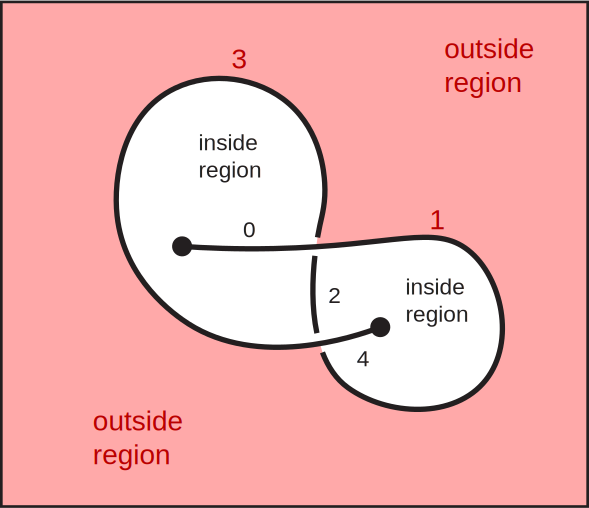
\includegraphics[scale=.35]{labeled_bifoil.pdf}
\caption{Labeled planar knotoid diagram corresponding to the PD code \lstinline{PD[X[2,r[1],r[3],0],X[r[1],4,2,r[3]]}.}\label{fig:labbif}
\end{figure}


Example of PD code for a knotoid diagram on the sphere (Figure~\ref{fig:labexamples} left):
\begin{lstlisting}
PD[
X[0,3,1,4],
X[4,1,5,2],
X[2,5,3,6]
];
\end{lstlisting}
It can also be written one line
\begin{lstlisting}
PD[X[0,3,1,4],X[4,1,5,2],X[2,5,3,6]];
\end{lstlisting}
Example of PD code for a knotoid diagram on the plane  (Figure~\ref{fig:labexamples} right):
\begin{lstlisting}
PD[
X[0,5,r[1],r[6]],
X[r[4],r[1],5,2],
X[7,2,8,3],
X[3,r[6],r[4],7]
];
\end{lstlisting}
and in one line
\begin{lstlisting}
PD[X[0,5,r[1],r[6]],X[r[4],r[1],5,2],X[7,2,8,3],X[3,r[6],r[4],7]];
\end{lstlisting}
Example of PD code for a knot diagram:
\begin{lstlisting}
PD[
X[0,3,1,4],
X[4,1,5,2],
X[2,5,3,0]
];
\end{lstlisting}
and in one line
\begin{lstlisting}
PD[X[0,3,1,4],X[4,1,5,2],X[2,5,3,0]];
\end{lstlisting}
\begin{figure}[t]
\centering
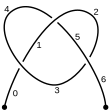
\includegraphics[scale=.35]{labeled_ex1.pdf}
\hspace*{2cm}
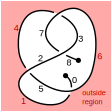
\includegraphics[scale=.35]{labeled_ex2.pdf}
\caption{Left: Labeled knotoid diagram corresponding to the PD code \lstinline{PD[X[0,3,1,4],X[4,1,5,2],X[2,5,3,6]]}. Right: Labeled knotoid diagram on the plane corresponding to the PD code \lstinline{PD[X[0,5,r[1],r[6]],X[r[4],r[1],5,2],X[7,2,8,3],X[3,r[6],r[4],7]]}.}\label{fig:labexamples}
\end{figure}

{\it Knoto-ID} also accept files with multiple diagrams. An example with two knotoid diagrams on the sphere:
\begin{lstlisting}
PD[X[3,1,4,0],X[1,5,2,4],X[5,3,6,2]];
PD[X[0,3,1,4],X[4,1,5,2],X[2,5,3,6]];
\end{lstlisting}
or simply concatenated in one line
\begin{lstlisting}
PD[X[3,1,4,0],X[1,5,2,4],X[5,3,6,2]];PD[X[0,3,1,4],X[4,1,5,2],X[2,5,3,6]];
\end{lstlisting}

The semicolons are not necessary and the following is also a valid list of diagrams
\begin{lstlisting}
PD[X[3,1,4,0],X[1,5,2,4],X[5,3,6,2]]PD[X[0,3,1,4],X[4,1,5,2],X[2,5,3,6]]
\end{lstlisting}

Finally, diagrams without crossings are allowed (Figure~\ref{fig:labempty}):
\begin{lstlisting}
PD[]
\end{lstlisting}

\begin{figure}[t]
\centering
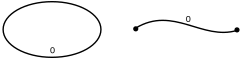
\includegraphics[scale=.35]{labeled_empty.pdf}
\caption{Left: Labeled knot diagram corresponding to the empty PD code \lstinline{PD[]}. Right: Labeled knotoid diagram corresponding to the empty PD code \lstinline{PD[]}.}\label{fig:labempty}
\end{figure}

\subsubsection{\label{sec:format:gauss}Knot(oid) diagrams (Extended Gauss code)}
Input and output format used to encode knot or knotoid diagrams based on the  extended Gauss codes\cite{gabrov,guka}. Extended gauss codes allows to encode knots and knotoid diagrams on the sphere and have the following form:
\[
\mbox{Gauss code} = \underbrace{\mbox{Crossings}}_{\mbox{first part}} \ \underbrace{\mbox{Signs}}_{\mbox{second part}}
\]

The {\bf first part} is a sequence of the crossings  of the diagram that is obtained by travelling around it, starting from one end and proceeding to the other, and labeling the crossings as we meet them (using strictly increasing non-negative integers). If we meet an undercrossing we note the crossing with a ``-'' sign, while if we meet an overcrossing we note it with a ``+'' sign. Note that each crossing is met twice in this trip and so each crossing will appear with both signs in the sequence. Therefore the length of this sequence is $2n$, where $n$ is the number of crossings. The case of knots is similar. The only difference is that we start the trip around the diagram from any arbitrary point. Note that different choices of starting points may yield different codes however, all codes will represent the same diagram. \\

The {\bf second part} is a sequence of the signs of each of the crossings of the diagram (Figure~\ref{crossings_v2}). Without it, the Gauss code represents a diagram up to its mirror image. The length of this sequence is $n$.\\

\begin{figure}[t]
\centering
\subfloat[]{
 \raisebox{-.1cm}{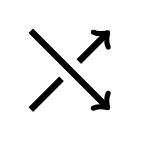
\begin{tikzpicture}[scale=.5]
\draw [line width=0.8mm]  (-1,-1)-- (-0.22,-0.22);
\draw  [line width=0.8mm](-1,1)--(0,0);
\draw  [line width=0.8mm] (0.22,0.22) -- (1,1)[->];
\draw [line width=0.8mm]   (0,0) -- +(1,-1)[->];
\end{tikzpicture}}}   \hspace{3cm}
\subfloat[]{ \raisebox{-.1cm}{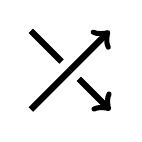
\begin{tikzpicture}[scale=.5]
\draw  [line width=0.8mm] (-1,-1)-- (0,0) ;
\draw [line width=0.8mm] (-1,1)--(-0.22,0.22);
\draw [line width=0.8mm] (0,0) -- (1,1)[->];
\draw [line width=0.8mm]   (0.22,-0.22) -- +(.8,-.8)[->];
\end{tikzpicture}}}
\caption{A positive crossing with sign +1 (a) and a negative crossing with sign -1 (b).}\label{crossings_v2}
\end{figure}

For example, the knotoid diagram in Figure~\ref{fig:gc_example1} (left) corresponds to the following extended Gauss code:
\begin{lstlisting}
  -1 2 -3 1 -2 3 ---
\end{lstlisting}
\begin{figure}[t]
\centering
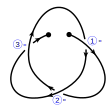
\includegraphics[width=0.25\textwidth]{gc_example2.pdf}\hspace{1cm}
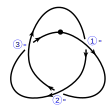
\includegraphics[width=0.25\textwidth]{gc_example3.pdf}
\caption{A knotoid diagram on the sphere and a knot diagram corresponding to the extended Gauss code \lstinline{-1 2 -3 1 -2 3 ---}. Crossing labels and signs are shown in blue.}\label{fig:gc_example1}
\end{figure}
Another example is the knotoid diagram shown in Figure~\ref{fig:gc_example4}, which corresponds to the following extended Gauss code:
\begin{lstlisting}
  1 -2 3 -1 -4 -5 2 -3 5 4 +++-+
\end{lstlisting}
\begin{figure}[t]
\centering
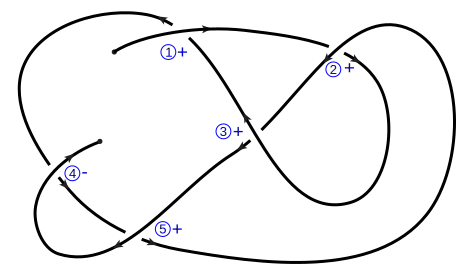
\includegraphics[width=0.6\textwidth]{gc_example5.pdf}
\caption{A labeled knotoid diagram corresponding to the extended Gauss code \lstinline{1 -2 3 -1 -4 -5 2 -3 5 4 +++-+}. Crossing labels and signs are shown in blue.}\label{fig:gc_example4}
\end{figure}

Except for pure knotoids, it is not possible to know whether a diagram is open or closed based only on its extended Gauss code. For example, both the knotoid diagram and the knot diagram in Figure~\ref{fig:gc_example1} correspond to the same extended Gauss code. Therefore, when loading a diagram from a Gauss code, one has to additionally specify whether it is open or closed using option \lstinline{--closure-method=open} (open diagram) or \lstinline{--closure-method=direct} or \lstinline{rays} (closed diagram). 


This form of extended Gauss codes cannot be used for planar diagrams as the information on which arcs touch the outside region is missing. For example, both knotoids diagrams in Figure~\ref{fig:gc_example2} correspond to the same extended Gauss code \lstinline{-1 2 -3 1 -2 3 ---}.
\begin{figure}[t]
\centering
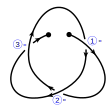
\includegraphics[width=0.25\textwidth]{gc_example2.pdf}\hspace{1cm}
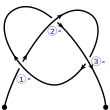
\includegraphics[width=0.25\textwidth]{gc_example1.pdf}
\caption{Two knotoid diagrams corresponding to the extended Gauss code \lstinline{-1 2 -3 1 -2 3 ---}. Crossing labels and signs are shown in blue.}\label{fig:gc_example2}
\end{figure}

To overcome this limitation, Knoto-ID accepts a modified version of the extended Gauss code, which allows the encoding of planar and spherical knotoid diagrams as well as knot diagrams. Such a code has the following form:
\[
\mbox{Gauss code} = \underbrace{\mbox{Crossings}}_{\mbox{first part}} \ \underbrace{\mbox{Signs}}_{\mbox{second part}} \ \underbrace{\mbox{Outside arcs}}_{\mbox{third part}}
\]

The {\bf first part} and {\bf second part} encode information on the crossings, as described previously.\\

The {\bf third part} allows the proper encoding of a planar knotoid diagram. It consists in a list of arc labels corresponding to the arcs of the diagram that are adjacent to the outside region of the diagram. This part has no fixed length. Note that arcs must be labeled with integer numbers, starting from 0 for the first arc and increasing by steps of 1 for each subsequent arc that is met when traveling along the curve.\\


For example, the knotoid diagram in Figure~\ref{fig:gc_example3} corresponds to the following extended Gauss code:
\begin{lstlisting}
  1 -2 3 -1 -4 -5 2 -3 5 4 +++-+ 0 3 4 5 8 10
\end{lstlisting}
\begin{figure}[t]
\centering
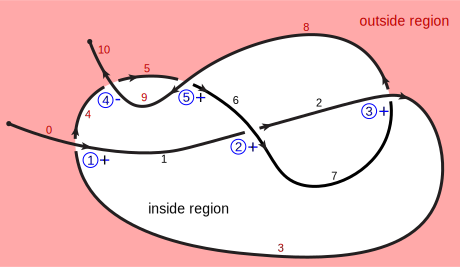
\includegraphics[width=0.6\textwidth]{gc_example4.pdf}
\caption{Labeled knotoid diagram corresponding to the extended Gauss code \lstinline{1 -2 3 -1 -4 -5 2 -3 5 4 +++-+ 0 3 4 5 8 10}. Crossing labels and signs are shown in blue. Arc labels are shown in red for arcs adjacent to the outside region and black for internal arcs.}\label{fig:gc_example3}
\end{figure}


Notes:
\begin{itemize}
\item For diagrams without crossings (Figure~\ref{fig:labempty}), the special keyword \lstinline{empty_diagram} is used.
\item When specifying whether a diagram is open or closed (with \lstinline{--closure-method}) care must be taken to avoid unrealisable diagrams. Two typical sources of mismatch between diagram topology and the choice of closure are:
\begin{itemize}
\item Closing a pure knotoid diagram. For example, the knotoid diagram in Figure~\ref{fig:labbif} with extended Gauss code \lstinline{1 -2 -1 2 ++ 1 3} cannot be closed without creating additional crossings. Note that {\it Knoto-ID} may read such a Gauss code without detecting that it does not correspond to realisable knot(oid) diagram. However this will lead to unpredictable output.
\item  Closing a planar knotoid diagram with its last endpoint in the outside region. For example, in the knotoid diagram shown in Figure~\ref{fig:gc_example3}, the last endpoint is outside and arc 10 appears in the extended Gauss code \lstinline{1 -2 3 -1 -4 -5 2 -3 5 4 +++-+ 0 3 4 5 8 10}. If we ask {\it Knoto-ID} to consider this diagram closed, it will complain that arc 10 does not exist ( arc 10 is merged arc 0 when closing the diagram).
\end{itemize}
\item While the labeling of arcs is very strict (starting from 0, increasing by steps of 1 when following the curve), labeling of nodes is more flexible. The only requirements are that node labels are non negative integer, and that the label increase when following the curve and meeting a crossing for the time.
All the following Gauss code correspond to the diagram shown in Figure~\ref{fig:gc_example3} (although with different labeling of the crossings):
\begin{lstlisting}
  1 -2 3 -1 -4 -5 2 -3 5 4 +++-+ 0 3 4 5 8 10
\end{lstlisting}
\begin{lstlisting}
  0 -1 2 -0 -3 -4 1 -2 4 3 +++-+ 0 3 4 5 8 10
\end{lstlisting}
but also
\begin{lstlisting}
  0 -5 7 -0 -10 -12 5 -7 12 10 +++-+ 0 3 4 5 8 10
\end{lstlisting}
Note that {\it Knoto-ID} relabels the crossings when loading a diagram from an extended Gauss code. Therefore the crossing labels in output may not correspond to the labels used in input. 
\item When reading an extended Gauss code, {\it Knoto-ID} replaces the following characters by blank space: \lstinline{[}, \lstinline{]}, \lstinline{(}, \lstinline{)}, \lstinlineT{\{}, \lstinlineT{\}}, \lstinline{,} and \lstinline{;}. As a consequence, the input format is quite flexible and all the following expressions are valid extended Gauss codes representing the knotoid diagram in  Figure~\ref{fig:gc_example2}:
\begin{lstlisting}
  {1,-2,3,-1,-4,-5,2,-3,5,4} {+++-+} {0,3,4,5,8,10}
\end{lstlisting}
\begin{lstlisting}
  (1 -2 3 -1 -4 -5 2 -3 5 4) (+ + + - +) (0 3 4 5 8 10)
\end{lstlisting}
\begin{lstlisting}
  1,-2,3,-1,-4,-5,2,-3,5,4,+,+,+,-,+,0,3,4,5,8,10
\end{lstlisting}
\end{itemize}

{\it Knoto-ID} also accept files with multiple diagrams, with one extended Gauss code per line. An example with two diagrams:
\begin{lstlisting}
1 -2 3 -1 2 -3 +++  
-1 2 -3 1 -2 3 ---
\end{lstlisting}



\subsubsection{\label{sec:format:multiprojection:jones}Distribution of polynomials}
Output format used to characterize the distribution of polynomials obtained with multiple projections. This is a tab separated format with 2 mandatory columns (frequency and polynomial) and 1 optional column (knot or knotoid type).
The first row is a header (starting with \#) specifying the label of each column.
In each subsequent row, the entry in column frequency is the fraction of all projections that gave the corresponding polynomial, followed optionally by the knot or knotoid type corresponding to the polynomial. Note that if weights were associated with the projections\footnote{see section ``\ref{sec:format:projections} \nameref{sec:format:projections}'' for more details.}, the column frequency contains the weighted fraction.

Example, without knot type:
\begin{lstlisting}
#frequency  polynomial
0.9         - A^(-16) + A^(-12) + A^(-4)
0.1         + 1
\end{lstlisting}
Example, with knot type:
\begin{lstlisting}
#frequency  knot_type  polynomial
0.7         3_1R       - A^(-16) + A^(-12) + A^(-4)
0.3         0_1        + 1
\end{lstlisting}



\subsubsection{\label{sec:format:multiprojection:diagrams}List of projections with polynomials and knot(oid) diagrams}
Tab separated output format with 5 columns (x, y, z coordinates of the projection direction, polynomial invariant and knot(oid) diagram) and  1 optional column (knot or knotoid type).
The first row is a header (starting with \#) specifying the label of each column.
With the optional column for the knot(oid) type, each subsequent row corresponds to a single projection direction (columns 1 to 3) together with the knot(oid) type (column 4), the polynomial (column 5) and PD code\footnote{see section ``\ref{sec:format:pd} \nameref{sec:format:pd}'' for more information on the file format.} or extended Gauss code\footnote{see section ``\ref{sec:format:gauss} \nameref{sec:format:gauss}'' for more information on the file format.} for the knot(oid) diagram (column 6) obtained from this projection.

Without the optional column for the knot(oid) type, the polynomial is given in column 4 and the PD code or extended Gauss code for the knot(oid) diagram is in column 5.


Example (without knot(oid) names):
\begin{lstlistingverysmall}
#projection.x  projection.y  projection.z  polynomial                    PD_code
0.483595       -0.85801      0.173072      - A^(-16) + A^(-12) + A^(-4)  PD[X[3,1,4,0],X[1,5,2,4],X[5,3,6,2]];
0.521928       -0.578265     0.627058      - A^(-16) + A^(-12) + A^(-4)  PD[X[3,1,4,0],X[1,5,2,4],X[5,3,6,2]];
0.898137       0.241849      0.367231      - A^(-16) + A^(-12) + A^(-4)  PD[X[7,0,8,1],X[4,2,5,1],X[2,6,3,5],X[6,4,7,3]];
-0.624015      0.596182      0.505146      - A^(-10) + A^(-6) + A^(-4)   PD[X[0,3,1,2],X[3,2,4,1]];
0.134038       -0.988518     -0.0697575    - A^(-16) + A^(-12) + A^(-4)  PD[X[5,1,6,0],X[1,5,2,4],X[2,8,3,7],X[6,4,7,3]];
\end{lstlistingverysmall}
Example (with knot(oid) names):
\begin{lstlistingverysmall}
#projection.x projection.y projection.z knotoid_type polynomial                   PD_code
0.483595      -0.85801     0.173072     k3.1o       - A^(-16) + A^(-12) + A^(-4)  PD[X[3,1,4,0],X[1,5,2,4],X[5,3,6,2]];
0.521928      -0.578265    0.627058     k3.1o       - A^(-16) + A^(-12) + A^(-4)  PD[X[3,1,4,0],X[1,5,2,4],X[5,3,6,2]];
0.898137      0.241849     0.367231     k3.1o       - A^(-16) + A^(-12) + A^(-4)  PD[X[7,0,8,1],X[4,2,5,1],X[2,6,3,5],X[6,4,7,3]];
-0.624015     0.596182     0.505146     k2.1        - A^(-10) + A^(-6) + A^(-4)   PD[X[0,3,1,2],X[3,2,4,1]];
0.134038      -0.988518    -0.0697575   k3.1o       - A^(-16) + A^(-12) + A^(-4)  PD[X[5,1,6,0],X[1,5,2,4],X[2,8,3,7],X[6,4,7,3]];
\end{lstlistingverysmall}
Example with extended Gauss code instead of PD code:
\begin{lstlistingverysmall}
#projection.x projection.y projection.z knotoid_type polynomial                    gauss_code
0.483595      -0.85801     0.173072     k3.1o       - A^(-16) + A^(-12) + A^(-4)   1 -2 3 -1 2 -3 +++
0.521928      -0.578265    0.627058     k3.1o       - A^(-16) + A^(-12) + A^(-4)   1 -2 3 -1 2 -3 +++
0.898137      0.241849     0.367231     k3.1o       - A^(-16) + A^(-12) + A^(-4)   1 2 -3 4 -2 3 -4 -1 -+++
-0.624015     0.596182     0.505146     k2.1        - A^(-10) + A^(-6) + A^(-4)    -1 2 1 -2 ++
0.134038      -0.988518    -0.0697575   k3.1o       - A^(-16) + A^(-12) + A^(-4)   1 -2 -3 4 2 -1 -4 3 ++++
\end{lstlistingverysmall}


\subsubsection{\label{sec:format:projections}List of projections}
Tab (or space) separated input format with 3 mandatory columns (x, y, z coordinates of the projection direction) and 1 optional column (weight)
The first row can optionally contain a header starting with \#.
Each subsequent row defines one projection direction with an optional weight (set to 1 if missing). The weight is used when evaluating the distribution of polynomials (the fraction of projections is replaced by a weighted fraction of projections)

Example:
\begin{lstlisting}
#projection.x  projection.y  projection.z  weight
0              0             1             1
0              1             0             1
1              0             0             1
0              0             -1            1
0              -1            0             1
-1             0             0             1
\end{lstlisting}



\subsubsection{\label{sec:format:namesdb}List of knot(oid) names}
Tab separated input format with 2 columns used to specify the correspondence between polynomials and knot(oid) names. Each row contains a knot or knotoid name in the first column and the corresponding polynomial in the second column.
While any string are accepted as a knot or knotoid name (as long as it does not contain a tab character), the polynomials must conform to the ``Polynomial'' format described in  section ``\ref{sec:format:polynomials} \nameref{sec:format:polynomials}''.

Two rows may contain the same polynomial with a different knot(oid) names. All knot(oid) names corresponding to the same polynomial will be concatenated  with a \lstinline{|} separator. For example, knots 6\_2R and 12n\_0025L have the same classical Jones polynomial $-1 + A^{-20} - 2 A^{-16} + 2 A^{-12} - 2 A^{-8} + 2 A^{-4} + A^4$ and the  corresponding knot name will be \lstinline{6_2R|12n_0025L}.


Example of list of knot names:
\begin{lstlisting}
0_1     1
3_1R    -A^(-16) + A^(-12) + A^(-4)
3_1L    A^4 + A^12 - A^16
4_1     1 + A^(-8) - A^(-4) - A^4 + A^8
5_1R    -A^(-28) + A^(-24) - A^(-20) + A^(-16) + A^(-8)
5_1L    A^8 + A^16 - A^20 + A^24 - A^28
5_2R    -A^(-24) + A^(-20) - A^(-16) + 2*A^(-12) - A^(-8) + A^(-4)
5_2L    A^4 - A^8 + 2*A^12 - A^16 + A^20 - A^24
6_1R    2 + A^(-16) - A^(-12) + A^(-8) - 2*A^(-4) - A^4 + A^8
6_1L    2 + A^(-8) - A^(-4) - 2*A^4 + A^8 - A^12 + A^16
6_2R    -1 + A^(-20) - 2*A^(-16) + 2*A^(-12) - 2*A^(-8) + 2*A^(-4) + A^4
6_2L    -1 + A^(-4) + 2*A^4 - 2*A^8 + 2*A^12 - 2*A^16 + A^20
6_3     3 - A^(-12) + 2*A^(-8) - 2*A^(-4) - 2*A^4 + 2*A^8 - A^12
\end{lstlisting}



\subsubsection{\label{sec:format:polynomials}Polynomials}
Polynomials are used both as input\footnote{section ``\ref{sec:format:namesdb} \nameref{sec:format:namesdb}''} and output\footnote{sections ``\ref{sec:format:multiprojection:jones} \nameref{sec:format:multiprojection:jones}'', ``\ref{sec:format:multiprojection:diagrams} \nameref{sec:format:multiprojection:diagrams}''.}.

Classical Jones polynomial and Jones polynomial for knotoids are univariate Laurent polynomials in variable $A$ with integer coefficients.
Turaev loop bracket polynomial is a bivariate Laurent polynomial in variables $A$ and $v$ with integer coefficients. See section ``\ref{sec:theory:jones} \nameref{sec:theory:jones}'' for more details.

For the file format, we consider the more general case of bivariate Laurent polynomial with integer coefficients. It should be written as a sum of monomials:
\[\sum_{n,m} C_{n,m}A^nv^m\text{ with }n,m,C_{n,m}\in\mathbb Z \]
Each monomial must be written using operators \lstinline{*} for multiplication and  \lstinline{^} for exponentiation:
\begin{lstlisting}
2*A^2*v^8
\end{lstlisting}

For clarity, exponents can be written between brackets
\begin{lstlisting}
2*A^(-4)*v^(2)
\end{lstlisting}
but it is not mandatory:
\begin{lstlisting}
2*A^-4*v^2
\end{lstlisting}
will also be interpreted as $2A^{-4}v^{2}$.

Terms with exponent 0 can be replaced by 1. For example \lstinline{2*A^(-4)*v^(0)} can be replaced by \lstinline{2*A^(-4)} and  \lstinline{2*A^(0)*v^(0)} can be replaced by \lstinline{2}.

Exponent 1 can be removed. For example \lstinline{2*v^(1)} can be replaced by \lstinline{2*v}.

Coefficient 1 can be removed for terms with non-zero exponent. For example  \lstinline{1*A^(-4)*v^(8)} can be replaced by \lstinline{A^(-4)*v^(8)} and   \lstinline{1*A^(-4)} can be replaced by \lstinline{A^(-4)}.

Finally, monomials must be combined with addition and subtraction operators (\lstinline{+} and \lstinline{-}):
\begin{lstlisting}
1 + A^(-8) - A^(-4) - A^4 + A^8
\end{lstlisting}
The first monomial can be prefixed by a unary sign operator
\begin{lstlisting}
-A^(-16) + A^(-12) + A^(-4)
\end{lstlisting}
Note that the combination of the binary addition or substraction operators with unary sign operator is not allowed: \lstinline{ + -A^2}, \lstinline{A^2 + -v^4} or \lstinline{A^2 - -v^4} will all generate an error.

Space character is allowed and can be used to improve readability but it is ignored.

Examples of valid polynomials:
\begin{lstlisting}
1
\end{lstlisting}
\begin{lstlisting}
-A^(-4) - 4*A^(-2)*v
\end{lstlisting}
\begin{lstlisting}
-A^2*v - A^4
\end{lstlisting}
\begin{lstlisting}
-A^-10 + A^-6 + A^-4
\end{lstlisting}
\begin{lstlisting}
1 + A^(-2) + v + A^(2)
\end{lstlisting}
\begin{lstlisting}
+A^(-8) + A^(-6)*v^(-4) - A^(-2)*v
\end{lstlisting}



  
\subsubsection{\label{sec:format:listsubchains}List of subchains}
Output format used by \lstinline{knotted_core} program to output the dominant knot(oid) of subchains of the input curve.
This is a tab separated format with 5 mandatory columns (first and last indices of the subchain, length of the subchain, frequency and polynomial)  and 1 optional column (Knot or knotoid type).
The first row is a header (starting with \#) specifying the label of each column.
Each subsequent row corresponds to one subchain, defined by its first and last indices (using zero-based indexing) as well as the length of the subchain (number of points). In addition, the corresponding dominant polynomial is given, together with its frequency (fraction of all projections that have the corresponding polynomial). Optionally, the Knot or knotoid type corresponding to the polynomial can also be given.

Each subchain is defined by a first index  and a length. Although not necessary to define the subchain, its last index is also given for completeness. Given a first index $i_1$, a length $l$ and a last index $i_2:=i_1+l-1{\rm\ mod\ } N$, the subchain is defined by the ordered set of points of the input curve with indices:
\[\{i_1{\rm\ mod\ } N,(i_1+1){\rm\ mod\ } N,\cdots,(i_1+l-1){\rm\ mod\ } N\}\]
where N is the number of points in the input curve (See Figures~\ref{fig:subchains:open} and \ref{fig:subchains:closed}).  
\begin{figure}[t]
\centering
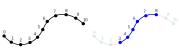
\includegraphics[width=0.6\textwidth]{subchains_open.pdf}
\caption{Left: open input curve with $N=11$ points. Right: a subchain with first index $i_1=3$, length $l=6$ and last index $i_2=8$ (blue).}\label{fig:subchains:open}
\end{figure}
\begin{figure}[t]
\centering
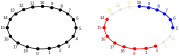
\includegraphics[width=0.6\textwidth]{subchains_closed.pdf}
\caption{left: closed input curve with $N=19$ points. Right: a subchain with first index $i_1=5$, length $l=6$ and last index $i_2=10$ (blue), and a  subchain with first index $i_1=14$, length $l=8$ and last index $i_2=2$ (red).}\label{fig:subchains:closed}
\end{figure}

Note: by definition, $l>N$ corresponds to the full input curve closed with direct closure.


Example for an open chain, without knot(oid) type:
\begin{lstlisting}
#index_first  index_last  length  frequency  polynomial
11            51          41      0.7        - A^(-10) + A^(-6) + A^(-4)
12            52          41      0.75       - A^(-16) + A^(-12) + A^(-4)
13            52          40      0.85       - A^(-16) + A^(-12) + A^(-4)
14            52          39      0.75       - A^(-16) + A^(-12) + A^(-4)
\end{lstlisting}

Example for a closed chain (with $N=111$ points), with knot type:
\begin{lstlisting}
#index_first  index_last  length  frequency  knot_type  polynomial
22            110         89      0.8        3_1R       - A^(-16) + A^(-12) + A^(-4)
22            0           90      0.5        3_1R       - A^(-16) + A^(-12) + A^(-4)
23            1           90      0.6        3_1R       - A^(-16) + A^(-12) + A^(-4)
22            79          58      0.8        3_1R       - A^(-16) + A^(-12) + A^(-4)
23            23          112     1          3_1R       - A^(-16) + A^(-12) + A^(-4)
\end{lstlisting}
Note that the length of last subchain is bigger than the number of input points, therefore the last subchain corresponds to the full input curve (with direct closure).

\subsubsection{\label{sec:format:xyzdiagrams}xyz format for knot(oid) diagrams} 
Tab (or space) separated output format with 4 columns corresponding to x, y, z coordinates and a label.
The first row is a header (starting with \#) specifying the label of each column.
Each subsequent row corresponds to a point of the curve. Consecutive points (rows) will be connected by a straight line. Note that consecutive lines may have the same x, y, z coordinates.
This format is used by \lstinline{convert_diagram} to output planar represenations of knot(oid) diagrams in the xy plane. The z coordinate ranges from -1 to +1 and is used to specify which arc is above ($z>0$) or below ($z<0$) at each crossing.

The following example corresponds to a knot diagram with two arcs and one crossing:
\begin{lstlisting}
#x y z label
0.728017   0.387851      0.698611   Arc_0
0.960894   0.511916      0.358889   Arc_0
1.02482    0.255915      0          Arc_0
1.02482    0.255915      0          Arc_0
1.08874    -8.68623e-05  -0.358889  Arc_0
0.824876   -6.58107e-05  -0.698611  Arc_0
0.824876   -6.58107e-05  -0.698611  Crossing_0
0          0             -1         Crossing_0
-0.824876  3.29053e-05   -0.698611  Crossing_0
-0.824876  3.29053e-05   -0.698611  Arc_1
-1.08874   4.34311e-05   -0.358889  Arc_1
-1.02481   -0.255956     0          Arc_1
-1.02481   -0.255956     0          Arc_1
-0.960873  -0.511954     0.358889   Arc_1
-0.728001  -0.38788      0.698611   Arc_1
-0.728001  -0.38788      0.698611   Crossing_0
0          0             1          Crossing_0
0.728017   0.387851      0.698611   Crossing_0
\end{lstlisting}

\clearpage
